\documentclass[11pt]{easymemo3}

%\SectionNumber
%\BlackAndWhite
\usepackage{lscape}

\begin{document}


\MakeTitle{2024.11.5}{対称操作}{明大理工 楠瀬博明}


\section{結晶の対称操作}

\subsection{結晶群}

長さを変えずに点$\bm{r}$ (極性ベクトル)を点$\bm{r}'$に移す対称操作を、点群の対称操作という。
以下、記号$\bm{a}$は3次元の実数列ベクトルを意味するものとする\footnote{内積$\bm{a}\cdot\bm{b}$は行列積では$\bm{a}^{t}\bm{b}$, 二項積(dyadic)は$\bm{a}\bm{b}=\bm{a}\bm{b}^{t}$である。Braket表記では$\braket{a|b}$および$\ket{a}\bra{b}$。}。
点群の対称操作は、$n$回回転操作と空間反転操作の積で表される。
結晶の周期性と整合する対称操作は$n=1,2,3,4,6$に限られる。
これらの対称操作から構成される点群を結晶点群とよび、32種類ある。

結晶点群に時間反転操作を加えた結晶点群を磁気点群とよび、122種類ある。
磁気点群は3つのタイプに分けられる。
\begin{itemize}
\item Type I: 時間反転操作を含まない磁気点群であり、32種類の結晶点群に等しい。
無色群 (colorless group)とも呼ばれる。
\item Type II: 結晶点群に純粋な時間反転操作を加えた点群であり、32種類ある。
灰色点群 (grey point group)と呼ばれる。
\item Type III: 時間反転操作と点群操作の合成操作を含む磁気点群であり、58種類ある。
黒白点群 (black-and-white point group)と呼ばれる。
\end{itemize}

結晶点群に単位格子の並進操作や部分並進操作を加えると230の空間群が得られる。
また、空間群に時間反転操作や部分並進と時間反転を組み合わせた操作を加えると1651の磁気空間群が得られる。
磁気空間群には磁気点群と同様にType I (230), Type II (230), Type-III (674) [black-and-white (ordinary Bravais lattice) group]があり、さらに時間反転+部分並進を含むType IV (517) [black-and white (black-and-white Bravais lattice) group]が加わる。
磁気空間群の表記には、国際表記との親和性が高いBNS (Belov-Neronova-Smirnova)表記と、空間群と反転操作の組で直接記述するOG (Opechowski-Guccione)表記がある。
後者は古い表記法で最近は前者が主に用いられる。
磁気空間群の頭文字は空間群と同様に格子系を表す。
Type IVでは、頭文字に時間反転並進を表す下添字をつける。
\begin{align}
&
a: (1/2,0,0),
\quad
b: (0,1/2,0),
\quad
c: (0,0,1/2)
\quad
(P格子)
\cr&
A: (1/2,0,0),
\quad
B: (0,1/2,0),
\quad
C: (0,0,1/2)
\quad(低心格子)
\cr&
I: (1/2,1/2,1/2)
\quad
(面心格子)
\cr&
S: (1/3,1/3,1/3)など
\quad
(格子依存、特殊方向)
\end{align}



\subsection{点群の対称操作}

Cartesian座標系($\bm{e}_{x},\bm{e}_{y},\bm{e}_{z}$; 正規直交系$\bm{e}_{i}\cdot\bm{e}_{j}=\delta_{ij}$, 右手系$(\bm{e}_{x}\times\bm{e}_{y})\cdot\bm{e}_{z}=1$)において、単位ベクトル$\bm{n}$軸まわりの$\theta$回転操作$\mathcal{R}(\theta;\bm{n})$を行うRodriguesの回転行列は、$l=1$の軌道角運動量演算子$\bm{l}$ ($\braket{j|l_{i}|k}=-i\epsilon_{ijk}$; $i,j,k=x,y,z$)を用いて
\begin{align}
&
C(\theta;\bm{n})=
e^{\theta K}
=1-\sin\theta\,K+(1-\cos\theta)K^{2},
\quad
K=i\bm{n}\cdot\bm{l}
=\begin{pmatrix}
0 & n_{z} & -n_{y} \\ -n_{z} & 0 & n_{x} \\ n_{y} & -n_{x} & 0
\end{pmatrix}
\end{align}
のように表される。
具体的に書き下すと
\begin{align}
   &
  C(\theta;\bm{n})=
  \begin{pmatrix}
    \cos \theta+n_{x}^{2}(1-\cos \theta)         & n_{x} n_{y}(1-\cos \theta)-n_{z} \sin \theta & n_{x} n_{z}(1-\cos \theta)+n_{y} \sin \theta \\
    n_{x} n_{y}(1-\cos \theta)+n_{z} \sin \theta & \cos \theta+n_{y}^{2}(1-\cos \theta)         & n_{y} n_{z}(1-\cos \theta)-n_{x} \sin \theta \\
    n_{x} n_{z}(1-\cos \theta)-n_{y} \sin \theta & n_{y} n_{z}(1-\cos \theta)+n_{x} \sin \theta & \cos \theta+n_{z}^{2}(1-\cos \theta)
  \end{pmatrix}.
  \label{eq:rotmat}
\end{align}
また、空間反転操作$\mathcal{P}$を行う行列は
\begin{align}
  P=
  \begin{pmatrix}
    -1 & 0 & 0 \\ 0 & -1 & 0 \\ 0 & 0 & -1
  \end{pmatrix}
\end{align}
である。
$C_{\bm{n}}(\theta)$の行列式は$1$、固有値は($1$, $e^{+i\theta}$, $e^{-i\theta}$)、$I$の行列式は$-1$である。
これらを任意に組み合わせた対称操作$W$により、点$\bm{r}=(r_x,r_y,r_z)^{t}$が$\bm{r}'=(r_x',r_y',r_z')^{t}$ ($t$は転置を表す)に移される。
\begin{align}
\bm{r}'=W\bm{r}.
\end{align}

点群の対称操作には、恒等操作$E$、$\bm{n}$軸に垂直な平面に関する鏡映操作$\sigma_{\bm{n}}$、$\bm{n}$軸まわりの$n$回回転操作$C_{n}(\bm{n})$、回反操作$\bar{C}_{n}(\bm{n})$、回鏡操作$S_{n}(\bm{n})$がある。
これらは、上述したように回転操作と反転操作の組み合わせで表現できる。
\begin{align}
&
E\equiv C(0;\bm{n})
\\&
C_{n}(\bm{n})\equiv C(2\pi/n;\bm{n})
\\&
  \bar{C}_{n}(\bm{n})\equiv PC(\frac{2\pi}{n};\bm{n})=-C(\frac{2\pi}{n};\bm{n})
\\&
  \sigma_{\bm{n}}=\bar{C}_{2}(\bm{n})
  =\begin{pmatrix}
    1-2n_x^2     & -2n_{x}n_{y} & -2n_{x}n_{z} \\
    -2n_{x}n_{y} & 1-2n_y^2     & -2n_{y}n_{z} \\
    -2n_{x}n_{z} & -2n_{y}n_{z} & 1-2n_z^2
  \end{pmatrix}
\\&
  S_{n}(\bm{n})\equiv \sigma_{\bm{n}}C_{n}({\bm{n}})=-C(\frac{2\pi}{n}+\pi;\bm{n}).
\end{align}

以上の定義より
\begin{align}
  P=-E=S_{2},
  \quad
  S_{3}(\bm{n})=PC_{-6}(\bm{n}),
  \quad
  S_{4}(\bm{n})=PC_{-4}(\bm{n}),
  \quad
  S_{6}(\bm{n})=PC_{-3}(\bm{n})
\end{align}
の関係がある。
回転操作を具体的に書き下すと
\begin{align}
      &
  C_2(x)=\begin{pmatrix}
    1 & 0  & 0  \\
    0 & -1 & 0  \\
    0 & 0  & -1
  \end{pmatrix},
  \quad
  C_2(y)=\begin{pmatrix}
    -1 & 0 & 0  \\
    0  & 1 & 0  \\
    0  & 0 & -1
  \end{pmatrix},
  \quad
  C_2(z)=\begin{pmatrix}
    -1 & 0  & 0 \\
    0  & -1 & 0 \\
    0  & 0  & 1
  \end{pmatrix},
  \cr &
  C_4(x)=\begin{pmatrix}
    1 & 0 & 0  \\
    0 & 0 & -1 \\
    0 & 1 & 0
  \end{pmatrix},
  \quad
  C_4(y)=\begin{pmatrix}
    0  & 0 & 1 \\
    0  & 1 & 0 \\
    -1 & 0 & 0
  \end{pmatrix},
  \quad
  C_4(z)=\begin{pmatrix}
    0 & -1 & 0 \\
    1 & 0  & 0 \\
    0 & 0  & 1
  \end{pmatrix},
  \cr &
  C_3(xyz)=\begin{pmatrix}
    0 & 0 & 1 \\
    1 & 0 & 0 \\
    0 & 1 & 0
  \end{pmatrix},
  \quad
  C_3(xy\bar{z})=\begin{pmatrix}
    0  & 1 & 0  \\
    0  & 0 & -1 \\
    -1 & 0 & 0
  \end{pmatrix},
  \quad
  C_3(x\bar{y}z)=\begin{pmatrix}
    0 & -1 & 0  \\
    0 & 0  & -1 \\
    1 & 0  & 0
  \end{pmatrix},
  \cr &
  C_3(\bar{x}yz)=\begin{pmatrix}
    0  & -1 & 0 \\
    0  & 0  & 1 \\
    -1 & 0  & 0
  \end{pmatrix},
  \quad
  C_6(z)=\begin{pmatrix}
    \frac{1}{2}        & -\frac{\sqrt{3}}{2} & 0 \\
    \frac{\sqrt{3}}{2} & \frac{1}{2}         & 0 \\
    0                  & 0                   & 1
  \end{pmatrix},
  \quad
  C_3(z)=[C_{6}(z)]^{2}.
\end{align}

\subsection{並進操作}

結晶では、上記の点群対称操作に基本格子ベクトル$(\bm{a}_{1},\bm{a}_{2},\bm{a}_{3})$の整数倍の並進操作($\bm{R}_{\bm{m}}=m_{1}\bm{a}_{1}+m_{2}\bm{a}_{2}+m_{3}\bm{a}_{3}$)や単位格子内の部分並進操作$\bm{w}$が加わる。
結晶点群操作に並進操作を加えた群を(結晶)空間群とよび、230種類ある。
部分並進操作(螺旋操作screwまたは映進操作glide)を含まない空間群をシンモルフィック群、含む空間群をノンシンモルフィック群という。

\subsection{時間反転操作}
時間反転操作は「'」記号で表され、磁気的な量(磁気多極子、磁気トロイダル多極子)の符号を反転させる操作である。

\section{結晶の座標軸}

\subsection{基本並進ベクトル}

基本並進ベクトル($\bm{a}_{1}$, $\bm{a}_{2}$, $\bm{a}_{3}$)を次のように(長さ$a,b,c$と角度$\alpha,\beta,\gamma$)により表す。
\begin{align}
      &
  \bm{a}_{1}=a\,\bm{e}_{x},
  \cr &
  \bm{a}_{2}=b\left[\cos\gamma \bm{e}_{x}+\sqrt{1-\cos^{2}\gamma} \bm{e}_{y}\right],
  \cr &
  \bm{a}_{3}=c\left[\cos\beta\bm{e}_{x}+\frac{\cos\alpha-\cos\beta\cos\gamma}{\sqrt{1-\cos^{2}\gamma}}\bm{e}_{y}+\frac{s}{\sqrt{1-\cos^{2}\gamma}}\bm{e}_{z}\right],
  \cr & \quad
  s=\sqrt{1-\cos^{2}\alpha-\cos^{2}\beta-\cos^{2}\gamma+2\cos\alpha\cos\beta\cos\gamma}.
\end{align}
この基本並進ベクトル(それぞれ$a,b,c$軸)で囲まれる平行六面体を慣用単位格子(conventional cell)といい、この単位格子の繰り返しがBravais格子である。
単位格子の体積は$\Omega=\bm{a}_{1}\cdot(\bm{a}_{2}\times\bm{a}_{3})=abcs$である。

基本並進ベクトルをまとめて
\begin{align}
  A=\begin{pmatrix} \bm{a}_{1} & \bm{a}_{2} & \bm{a}_{3} \end{pmatrix}
  =\begin{pmatrix}
    a_{1x} & a_{2x} & a_{3x} \\
    a_{1y} & a_{2y} & a_{3y} \\
    a_{1z} & a_{2z} & a_{3z}
  \end{pmatrix},
\end{align}
のように表すと、実空間の任意の座標$\bm{r}$は
\begin{align}
  \bm{r}=x\bm{a}_{1}+y\bm{a}_{2}+z\bm{a}_{3}=A\bm{x},
  \quad
  \bm{x}=(x,y,z)^{t}
\end{align}
のように表される。
係数$(x,y,z)$を分率座標(fractional coordinate)という。

また、計量テンソルを
\begin{align}
  G=A^{t}A=
  \begin{pmatrix}
    \bm{a}_{1}\cdot\bm{a}_{1} & \bm{a}_{1}\cdot\bm{a}_{2} & \bm{a}_{1}\cdot\bm{a}_{3} \\
    \bm{a}_{2}\cdot\bm{a}_{1} & \bm{a}_{2}\cdot\bm{a}_{2} & \bm{a}_{2}\cdot\bm{a}_{3} \\
    \bm{a}_{3}\cdot\bm{a}_{1} & \bm{a}_{3}\cdot\bm{a}_{2} & \bm{a}_{3}\cdot\bm{a}_{3}
  \end{pmatrix}
  =
  \begin{pmatrix}
    a^{2}        & ab\cos\gamma & ac\cos\beta  \\
    ab\cos\gamma & b^{2}        & bc\cos\alpha \\
    ac\cos\beta  & bc\cos\alpha & c^{2}
  \end{pmatrix}
\end{align}
のように導入すると、内積を$\bm{r}_{1}\cdot\bm{r}_{2}=\bm{r}_{1}^{t}\bm{r}_{2}=\bm{x}_{1}^{t}G\bm{x}_{2}$のように分率座標を用いて表すことができる。
2点間の距離の自乗は$(\bm{r}_{1}-\bm{r}_{2})^{2}=\bm{x}_{1}^{t}G\bm{x}_{1}+\bm{x}_{2}^{t}G\bm{x}_{2}-2\bm{x}_{1}^{t}G\bm{x}_{2}$である。

\subsection{単位格子}

\begin{figure}[t!]
  \small
  \centering
  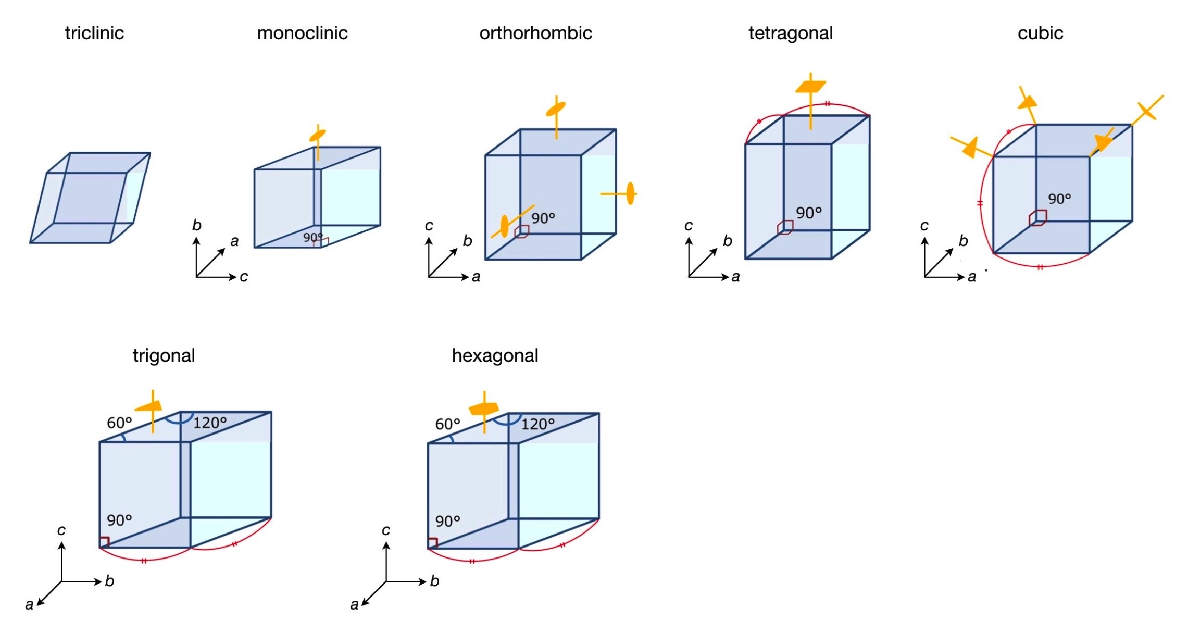
\includegraphics[width=14cm]{fig/crystal.eps}
  \caption{7つの晶系と必須対称要素。}
\label{fig:1}
\end{figure}

\begin{table}[h!]
  \caption{7つの晶系と14種のBravais格子および対応する点群(各晶系の先頭が最も対称性が高い)。三方晶に対するrhombohedral axes ($a=b=c$, $\alpha=\beta=\gamma$)は用いない。
  \label{tbl:1}}
  \begin{tabular}{lllll} \hline\hline
    結晶系         & 必須対称要素 & Bravais格子         & 単位格子の形状                                    & 点群                                              \\ \hline
    三斜晶         & $1$ or       & 三斜格子 ($aP$)     & $a\ne b\ne c$,                                    & $C_{\rm i}$, $C_{1}$                              \\
    (triclinic)    & $-1$         &                     & $\alpha\ne\beta\ne\gamma\ne 90^{\circ}$                                                               \\ \hline
    単斜晶         & $2$ or       & 単純単斜格子 ($mP$) & $a\ne b\ne c$,                                    & $C_{\rm 2h}$, $C_{\rm s}$, $C_{2}$                \\
    (monoclinic)   & $-2$ ($m$)   & 底心単斜格子 ($mC$) & $\alpha=\gamma= 90^{\circ}$, $\beta\ne90^{\circ}$                                                     \\
                   &              &                     & (unique axis $b$)                                                                                     \\ \hline
    直方晶         & $2$ (3つ) or & 単純直方格子 ($oP$) & $a\ne b\ne c$,                                    & $D_{\rm 2h}$, $D_{2}$, $C_{\rm 2v}$               \\
    (orthorhombic) & $-2$ (3つ)   & 体心直方格子 ($oI$) & $\alpha=\beta=\gamma= 90^{\circ}$                                                                     \\
                   &              & 底心直方格子 ($oC$)                                                                                                         \\
                   &              & 面心直方格子 ($oF$)                                                                                                         \\ \hline
    正方晶         & $4$ or       & 単純正方格子 ($tP$) & $a=b\ne c$,                                       & $D_{\rm 4h}$, $D_{4}$, $D_{\rm 2d}$,              \\
    (tetragonal)   & $-4$         & 体心正方格子 ($tI$) & $\alpha=\beta=\gamma= 90^{\circ}$                 & $C_{\rm 4v}$, $C_{\rm 4h}$, $S_{4}$, $C_{4}$      \\ \hline
    三方晶         & $3$ or       & 三方格子 ($hP$)     & $a=b\ne c$,                                       & $D_{\rm 3d}$, $D_{3}$, $C_{\rm 3v}$,              \\
    (trigonal)     & $-3$         & 稜面格子 ($hR$)     & $\alpha=\beta= 90^{\circ}$, $\gamma=120^{\circ}$  & $S_{6}$, $C_{3}$                                  \\
                   &              &                     & (hexagonal axes)                                  &                                                   \\ \hline
    六方晶         & $6$ or       & 六方格子 ($hP$)     & $a=b\ne c$,                                       & $D_{\rm 6h}$, $D_{6}$, $D_{\rm 3h}$,              \\
    (hexagonal)    & $-6$         &                     & $\alpha=\beta= 90^{\circ}$, $\gamma=120^{\circ}$  & $C_{\rm 6v}$, $C_{\rm 6h}$, $C_{\rm 3h}$, $C_{6}$ \\ \hline
    立方晶         & $3$ (4つ) or & 単純立方格子 ($cP$) & $a=b=c$,                                          & $O_{\rm h}$, $O$, $T_{\rm d}$,                    \\
    (cubic)        & $-4$ (4つ)   & 体心立方格子 ($cI$) & $\alpha=\beta=\gamma=90^{\circ}$                  & $T_{\rm h}$, $T$                                  \\
                   &              & 面心立方格子 ($cF$)                                                                                                         \\
    \hline\hline
  \end{tabular}
\end{table}

\begin{table}[h!]
\caption{7つの晶系の主軸・副軸・副副軸とCartesian座標系との関係。
\label{tbl:abc}}
\begin{tabular}{llllllll} \hline\hline
Crystal & $x$ & $y$ & $z$ & Primary & Secondary & Tertiary & Remark \\ \hline
triclinic & $[100]$ & - & - & - & - & - \\
monoclinic & - & $[010]$ & - & $[010]$ & - & - & unique axis $b$ \\
orthorhombic & $[100]$ & $[010]$ & $[001]$ & $[100]$ & $[010]$ & $[001]$ & \\
tetragonal & $[100]$ & $[010]$ & $[001]$ & $[001]$ & $\braket{100}$ & $\braket{110}$ & \\
trigonal & $[100]$ & $[120]$ & $[001]$ & $[001]$ & $\braket{100}$ & $\braket{120}$ & \\
hexagonal (rhombohedral) & $[100]$ & $[120]$ & $[001]$ & $[001]$ & $\braket{100}$ & $\braket{120}$ & hexagonal axes \\
cubic & $[100]$ & $[010]$ & $[001]$ & $\braket{001}$ & $\braket{111}$ & $\braket{110}$ \\ \hline\hline
\end{tabular}
\end{table}

慣用単位格子は7つの晶系(図\ref{fig:1})のいずれかに属し、32の結晶点群は表\ref{tbl:1}のように分類される。
座標系はITAに従い、表\ref{tbl:abc}にまとめておく。

各晶系に対する変換行列$A$は以下の通りである。
\begin{itemize}
\item 単斜晶(monoclinic) (主軸$\bm{a}_{2}$ ($y$)軸:標準セッティング)
\begin{align}
   &
  \alpha=\gamma=90^{\circ}
  \To
  A_{\rm m}=\begin{pmatrix}
    a & 0 & c\cos\beta \\
    0 & b & 0          \\
    0 & 0 & c\sin\beta
  \end{pmatrix}.
\end{align}
\item 直方晶(orthorhombic)、正方晶(tetragonal) ($a=b$)、立方晶(cubic) ($a=b=c$)
\begin{align}
   &
  \alpha=\beta=\gamma=90^{\circ}
  \To
  A_{\rm o}=\begin{pmatrix}
    a & 0 & 0 \\
    0 & b & 0 \\
    0 & 0 & c
  \end{pmatrix},
  \quad
  A_{\rm t}=\begin{pmatrix}
    a & 0 & 0 \\
    0 & a & 0 \\
    0 & 0 & c
  \end{pmatrix},
  \quad
  A_{\rm c}=\begin{pmatrix}
    a & 0 & 0 \\
    0 & a & 0 \\
    0 & 0 & a
  \end{pmatrix}.
\end{align}
\item 三方晶(trigonal)、六方晶(hexagonal)
\begin{align}
   &
  a=b,
  \quad
  \alpha=\beta=90^{\circ},
  \quad
  \gamma=120^{\circ}
  \To
  A_{\rm h}=\begin{pmatrix}
    a & -\frac{a}{2}        & 0 \\
    0 & \frac{\sqrt{3}a}{2} & 0 \\
    0 & 0                   & c
  \end{pmatrix}.
\end{align}
\end{itemize}


\subsection{座標軸の変換}

前節の基本並進ベクトル($\bm{a}_{1}$, $\bm{a}_{2}$, $\bm{a}_{3}$)とは異なる基本並進ベクトルを($\widetilde{\bm{a}}_{1}$, $\widetilde{\bm{a}}_{2}$, $\widetilde{\bm{a}}_{3}$)と表す。
両者の関係を
\begin{align}
  \widetilde{A}=
  \begin{pmatrix} \widetilde{\bm{a}}_{1} & \widetilde{\bm{a}}_{2} & \widetilde{\bm{a}}_{3} \end{pmatrix}
  =
  AP,
  \quad
  P=\begin{pmatrix}
    P_{11} & P_{12} & P_{13} \\
    P_{21} & P_{22} & P_{23} \\
    P_{31} & P_{32} & P_{33}
  \end{pmatrix}
\end{align}
と表す。
また、原点を$\bm{t}$だけ移動する操作を
\begin{align}
  \bm{t}=p_{1}\bm{a}_{1}+p_{2}\bm{a}_{2}+p_{3}\bm{a}_{3}=A\bm{p},
  \quad
  \bm{p}=(p_{1},p_{2},p_{3})^{t}
\end{align}
とする。
座標軸変換と原点移動をまとめて
\begin{align}
  \mathbb{P}=\begin{pmatrix}
    P          & \bm{p} \\
    \bm{o}^{t} & 1
  \end{pmatrix},
  \quad
  \mathbb{A}=\begin{pmatrix}
    A          & \bm{o} \\
    \bm{o}^{t} & 1
  \end{pmatrix}
\end{align}
とする。
ここで、$\bm{o}=(0,0,0)^{t}$とした。

任意の点$\bm{r}$を、2種の座標系で表すと
\[
  \begin{pmatrix} \bm{r} \\  1 \end{pmatrix}
  =\mathbb{A}\begin{pmatrix} \bm{x} \\ 1 \end{pmatrix},
  \quad
  \begin{pmatrix} \bm{r} \\  1 \end{pmatrix}
  =\begin{pmatrix} \tilde{x}\widetilde{\bm{a}}_{1}+\tilde{y}\widetilde{\bm{a}}_{2}+\tilde{z}\widetilde{\bm{a}}_{3}+\bm{t} \\ 1 \end{pmatrix}
  =\begin{pmatrix} A(P\widetilde{\bm{x}}+\bm{p}) \\ 1 \end{pmatrix}
  =
  \mathbb{A}\mathbb{P}\begin{pmatrix} \widetilde{\bm{x}} \\ 1 \end{pmatrix}
\]
より、2つの座標系の座標点$\bm{x}$, $\widetilde{\bm{x}}$の間の変換則が得られる。
\begin{align}
  \begin{pmatrix} \widetilde{\bm{x}} \\ 1 \end{pmatrix}=\mathbb{P}^{-1}\begin{pmatrix} \bm{x} \\ 1 \end{pmatrix}.
\end{align}

同様にして対称操作の変換則を求めよう。
ある対称操作$\mathcal{W}$によって
\begin{align}
  \begin{pmatrix} x' \\ y' \\ z' \\ 1 \end{pmatrix}
  =
  \begin{pmatrix}
    W_{11} & W_{12} & W_{13} & w_{1} \\
    W_{21} & W_{22} & W_{23} & w_{2} \\
    W_{31} & W_{32} & W_{33} & w_{3} \\
    0      & 0      & 0      & 1     \\
  \end{pmatrix}
  \begin{pmatrix} x \\ y \\ z \\ 1 \end{pmatrix}
  \To
  \begin{pmatrix} \bm{x}' \\ 1 \end{pmatrix}
  =\mathbb{W}
  \begin{pmatrix} \bm{x} \\ 1 \end{pmatrix},
  \quad
  \mathbb{W}
  =\begin{pmatrix} W & \bm{w} \\ \bm{o}^{t} & 1 \end{pmatrix}
\end{align}
のように$\bm{x}$が$\bm{x}'$に移されるとする。
この関係を2つの座標系に適用すると、対称操作の変換則が得られる。
\begin{align}
  \begin{pmatrix} \widetilde{\bm{x}}' \\ 1 \end{pmatrix}
  =\widetilde{\mathbb{W}}
  \begin{pmatrix} \widetilde{\bm{x}} \\ 1 \end{pmatrix}
  \To
  \begin{pmatrix} \bm{x}' \\ 1 \end{pmatrix}
  =\mathbb{P}\widetilde{\mathbb{W}}
  \mathbb{P}^{-1}\begin{pmatrix} \bm{x} \\ 1 \end{pmatrix}
  \To
  \widetilde{\mathbb{W}}=\mathbb{P}^{-1}\mathbb{W}\mathbb{P}.
\end{align}
特に、原点移動を伴わない変換($\bm{p}=0$)の場合
\begin{align}
  \widetilde{W}=P^{-1}WP^{},
  \quad
  \widetilde{\bm{w}}=P^{-1}\bm{w}.
\end{align}
原点移動のみの変換($P=1$)の場合
\begin{align}
  \widetilde{W}=W,
  \quad
  \widetilde{\bm{w}}=W\bm{p}+\bm{w}-\bm{p}.
\end{align}
例えば、主軸が$b$軸である座標系から$a$軸や$c$軸が主軸の座標系に移るには
\begin{align}
  P_{a}=\begin{pmatrix} 0 & 1 & 0 \\ 0 & 0 & 1 \\ 1 & 0 & 0 \end{pmatrix},
  \quad
  P_{c}=\begin{pmatrix} 0 & 0 & 1 \\ 1 & 0 & 0 \\ 0 & 1 & 0 \end{pmatrix},
  \quad\quad
  P_{b}=\begin{pmatrix} 1 & 0 & 0 \\ 0 & 1 & 0 \\ 0 & 0 & 1 \end{pmatrix}.
\end{align}

デカルト座標から分率座標への変換は$(\bm{a}_{1},\bm{a}_{2},\bm{a}_{3})\to(\bm{e}_{x},\bm{e}_{y},\bm{e}_{z})$, $(\widetilde{\bm{a}}_{1},\widetilde{\bm{a}}_{2},\widetilde{\bm{a}}_{3})\to(\bm{a}_{1},\bm{a}_{2},\bm{a}_{3})$ (ただし$a=b=c=1$)、すなわち$A\to1$, $P\to A$と読み替えればよいから、例えば三方晶や六方晶では
\begin{align}
P_{\rm h}=
\begin{pmatrix}
1 & -\frac{1}{2} & 0 \\
0 & \frac{\sqrt{3}}{2} & 0 \\
0 & 0 & 1
\end{pmatrix}.
\end{align}

以上の変換式を用いれば、例えば、三方晶や六方晶の分率座標で、対称操作$C_{6}(c)$や$C_{3}(c)$は
\begin{align}
  C_6(c)=P_{\rm h}^{-1}C_{6}(z)P_{\rm h}^{}=\begin{pmatrix}
    1 & -1 & 0 \\
    1 & 0  & 0 \\
    0 & 0  & 1
  \end{pmatrix},
  \quad
  C_3(c)=[C_{6}(c)]^{2}
\end{align}
となる。
同様に、$C_{2}(b)$は単斜晶の分率座標では
\begin{align}
  C_2(b)=P_{\rm m}^{-1}C_{2}(y)P_{\rm m}^{}=\begin{pmatrix}
    -1 & 0 & 0  \\
    0  & 1 & 0  \\
    0  & 0 & -1
  \end{pmatrix}.
\end{align}


\subsection{Primitive cell}

体積が最小となるような単位格子(primitive cell)の基本並進ベクトル$(\underline{\bm{a}}_{1},\underline{\bm{a}}_{2},\underline{\bm{a}}_{3})$を考える。
Bravais格子$(\bm{a}_{1},\bm{a}_{2},\bm{a}_{3})$からprimitiveな単純格子(P: simple lattice)、体心格子(I: body-centered lattice)、面心格子(F: face-centered lattice)への変換行列はそれぞれ以下のようになる。
\begin{align}
   &
  P_{\rm P}=\begin{pmatrix}
    1 & 0 & 0 \\
    0 & 1 & 0 \\
    0 & 0 & 1
  \end{pmatrix},
  \quad
  P_{\rm I}=\frac{1}{2}\begin{pmatrix}
    -1 & 1  & 1  \\
    1  & -1 & 1  \\
    1  & 1  & -1
  \end{pmatrix},
  \quad
  P_{\rm F}=\frac{1}{2}\begin{pmatrix}
    0 & 1 & 1 \\
    1 & 0 & 1 \\
    1 & 1 & 0
  \end{pmatrix}.
\end{align}
底心格子(A,B,C: base-centered lattice)の場合は
\begin{align}
   &
  P_{\rm A}=\frac{1}{2}\begin{pmatrix}
    2 & 0 & 0  \\
    0 & 1 & -1 \\
    0 & 1 & 1  \\
  \end{pmatrix},
  \quad
  P_{\rm B}=\frac{1}{2}\begin{pmatrix}
    1  & 0 & 1 \\
    0  & 2 & 0 \\
    -1 & 0 & 1 \\
  \end{pmatrix},
  \quad
  P_{\rm C}=\frac{1}{2}\begin{pmatrix}
    1 & -1 & 0 \\
    1 & 1  & 0 \\
    0 & 0  & 2
  \end{pmatrix}.
\end{align}
稜面格子では、rhombohedralセッティング($a=b=c$, $\alpha=\beta=\gamma$)は用いず、hexagonalセッティング($a=b$, $\alpha=\beta=90^{\circ}$, $\gamma=120^{\circ}$)のみを用いる。
\begin{align}
   &
  P_{\rm R}=\frac{1}{3}\begin{pmatrix}
    2 & -1 & -1 \\
    1 & 1  & -2 \\
    1 & 1  & 1
  \end{pmatrix}.
\end{align}

慣用単位格子は最小単位格子より大きいので、慣用単位格子の基本並進操作$\bm{p}_{\rm P}=(0,0,0)^{t}$に加えて、以下の「部分」並進操作を追加することで、Bravais格子の格子点が得られる。
\begin{itemize}
  \item 体心格子: $\bm{p}_{\rm I}=\frac{1}{2}(1,1,1)^{t}$
  \item 面心格子: $\bm{p}_{\rm F}=\frac{1}{2}(1,1,0)^{t}$, $\frac{1}{2}(1,0,1)^{t}$, $\frac{1}{2}(0,1,1)^{t}$
  \item 底心格子: $\bm{p}_{\rm A}=\frac{1}{2}(0,1,1)^{t}$, $\bm{p}_{\rm B}=\frac{1}{2}(1,0,1)^{t}$, $\bm{p}_{\rm C}=\frac{1}{2}(1,1,0)^{t}$
  \item 稜面格子: $\bm{p}_{\rm R}=\frac{1}{3}(2,1,1)^{t}$, $\frac{1}{3}(1,2,2)^{t}$
\end{itemize}



\subsection{対称操作の記号}

結晶点群や空間群の対称操作を以下のように文字列で表す。
並進操作は省略可。
\begin{itemize}
  \item 空間反転({\tt -})
  \item $n$回回転({\tt 2,3+/-,4+/-,6+/-})
  \item 鏡映({\tt m})
  \item 回転または鏡映軸[$n_1n_2n_3$] (基本格子ベクトルに対して)
  \item 並進[$t_1,t_2,t_3$] (基本格子ベクトルに対して)
  \item 時間反転({\tt '})
\end{itemize}
\begin{quote}
  略称 = 空間反転, $n$回回転, 鏡映, 軸, 時間反転 : 並進
\end{quote}

例
\begin{quote}
  \texttt{2[001]} = $2_{\,001}$,\quad
  \texttt{-3+[111]} = $-3^+_{\,111}$,\quad
  \texttt{3-[-1-11]} = $3^-_{\,-1-11}$,\quad
  \texttt{m[011]} = ${\rm m}_{011}$,\\
  \texttt{-3'+[111]} = $-3^+_{\,111}{}'$,\quad
  \texttt{m[010]:[0,1/2,1/2]} = $\{{\rm m}_{010}|0 \frac{1}{2} \frac{1}{2}\}$ など
\end{quote}


\subsection{結晶群の名称とセッティング}

\begin{figure}[t!]
  \small
  \centering
  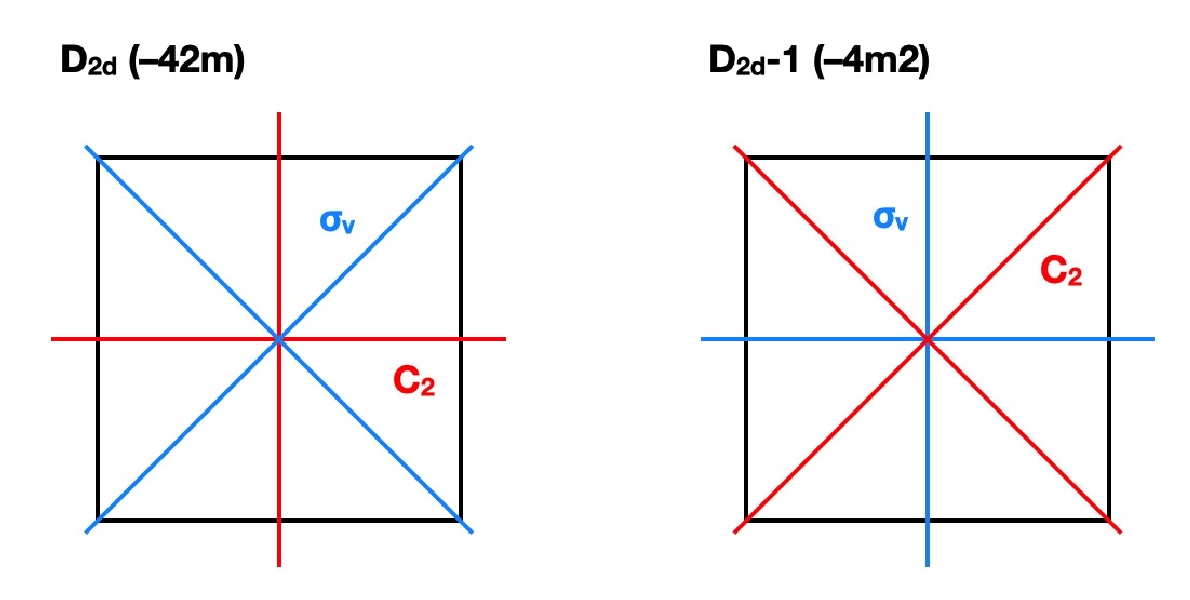
\includegraphics[width=7cm]{fig/setting_tet.eps}
  \caption{$D_{\rm 2d}$のセッティング(左が標準)。\label{fig:2}}
\end{figure}
\begin{figure}[t!]
  \small
  \centering
  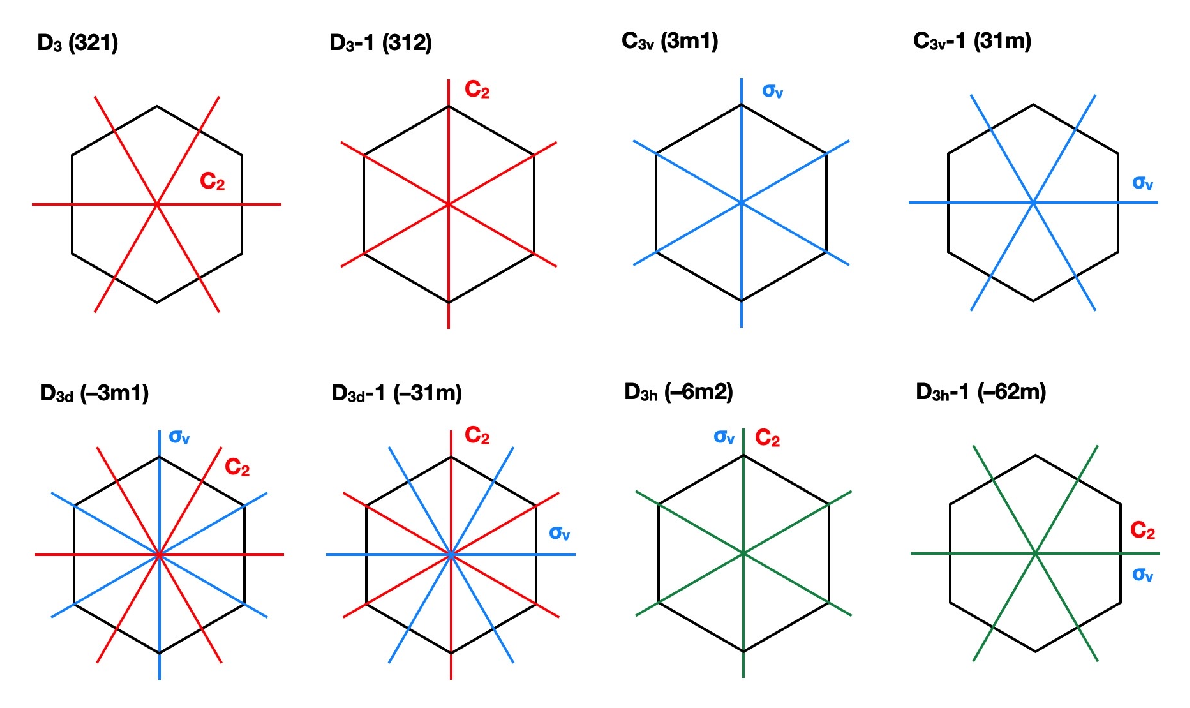
\includegraphics[width=12cm]{fig/setting_tri.eps}
  \caption{$D_{3},C_{\rm 3v},D_{\rm 3d},D_{\rm 3h}$のセッティング(左が標準)。\label{fig:3}}
\end{figure}


結晶群の名称としてSch\"{o}nflies記号($O_{\rm h}$, $O_{\rm h}^{5}$など)や国際表記(短縮形: $m{-}3m$, $Fm{-}3m$など)が用いられる。
軸や原点の取り方に複数のセッティングがあるが、標準セッティングは以下のとおりである。
\begin{itemize}
  \item 単斜晶: 主軸:$b$ ($y$)軸 (Cell Choice 1)
  \item 三方晶: hexagonal axes ($a=b$, $\alpha=\beta=90^{\circ}$, $\gamma=120^{\circ}$)
  \item 直方晶、正方晶、立方晶: 反転中心が原点 (Origin Choice 2)
\end{itemize}

直方晶($D_{\rm 2d}$)、三方晶、六方晶($D_{3},C_{\rm 3v},D_{\rm 3d},D_{\rm 3h}$)は副軸まわりの回転軸と鏡映面の取り方が2通りある。
図\ref{fig:2}, \ref{fig:3}に示すように、($-42m$), ($321$), ($3m1$) ($-3m1$), ($-6m2$)を標準セッティングとする。

\section{諸注意}

空間群から並進操作を取り除いた点群を得るには、Sch\"{o}nflies記号の上付の数字を削除すればよい。
ただし、上記のように副軸まわりの回転軸と鏡映面の取り方が2通りある場合は、対応する点群が標準セッティングではない場合があるので注意が必要である。
例えば、No.111 [$D_{2d}^{1}$, $P-42m$]$\to D_{2d}$ ($-42m$), No.115 [$D_{2d}^{5}$, $P-4m2$]$\to D_{2d}$-1 ($-4m2$)である。

空間群の対称操作から(部分)並進操作(「:」以降)を除いた点群操作の集合は、対応する結晶点群と順序も含めて一致するように選ばれている。

同様に、磁気空間群の対称操作から(部分)並進操作(「:」以降)を除いた点群操作の集合は、対応する磁気点群の操作と一致する。
ただし、重複する操作は取り除く必要がある。
このため、順序まで含めて一致するようには選ばれていない。

磁気点群の対称操作から時間反転操作「'」を除くと、対応する結晶点群の操作と一致する。
ただし、重複する操作は取り除く必要がある。
このため、順序まで含めて一致するようには選ばれていない。

磁気空間群の対称操作から時間反転操作「'」を除くと、対応する空間群の操作に加えて部分並進を伴う操作が残る場合がある。
BNSのNo表示(\#.\#)の最初の数字が空間群番号を表すので、対応する空間群の対称操作は、その番号を用いて参照する。
また、空間群ではprimitive$\to$conventional変換の際に適当な部分並進を加える必要があるが、磁気空間群の対称操作にはこれらは明示的に含まれているので、適当な部分並進を加える必要はない。


\newpage
\appendix


\section{対称操作の基礎}

\subsection{基底と表現(成分表示)}

対称操作$\mathcal{W}$に対して任意の状態$\ket{a}$は
\begin{align}
  \ket{a'}\equiv\mathcal{W}\ket{a}
\end{align}
のように変換する。
状態$\ket{a}$の完全正規直交基底系を$\{\ket{i}\}$とし、$\ket{a}$が基底の1つ$\ket{j}$であると考えると、基底自体の変換は
\begin{align}
  \ket{j'}=\mathcal{W}\ket{j}
  =\sum_{i}\ket{i}\braket{i|\mathcal{W}|j}
  =\sum_{i}\ket{i}W_{ij},
  \quad
  W_{ij}\equiv\braket{i|\mathcal{W}|j}
  \label{eq:59}
\end{align}
となる。
ここで、$W_{ij}$は基底$\{\ket{i}\}$に対する対称操作$\mathcal{W}$の表現行列の要素(成分)である。
一方、状態の成分は
\begin{align}
  a_{i}'\equiv\braket{i|a'}=\braket{i|\mathcal{W}|a}
  =\sum_{j}\braket{i|\mathcal{W}|j}\braket{j|a}
  =\sum_{j}W_{ij}a_{j}
\end{align}
のように変換される。

対称操作を施しても、基底の正規直交性が保たれることから
\begin{align}
  \braket{i'|j'}=\braket{i|\mathcal{W}^{\dagger}\mathcal{W}^{}|j}=\braket{i|j}=\delta_{ij}
  \To
  \mathcal{W}^{-1}=\mathcal{W}^{\dagger}
\end{align}
となるので、対称操作$\mathcal{W}$はユニタリーである。
表現行列の要素で表すと
\begin{align}
  (W^{-1})_{ij}=(W^{\dagger})_{ij},
  \quad
  (W^{\dagger})_{ij}=W_{ji}^{*},
  \quad
  \sum_{k}W_{ik}^{}W_{jk}^{*}=\delta_{ij}
\end{align}

次に、任意の1体演算子$\mathcal{A}$を考えよう。
まず、演算子を表すための基底は
\begin{align}
\ket{i'}\bra{j'}=\mathcal{W}\ket{i}\bra{j}\mathcal{W}^{\dagger}=\sum_{kl}\ket{k}\bra{l}W_{ki}W_{jl}^{\dagger}
\end{align}
のように変換する。
$\mathcal{A}$が任意の状態$\ket{a}$を用いて
\begin{align}
  \mathcal{A}=\sum_{ab}A_{ab}\ket{a}\bra{b}
\end{align}
のように表されるとすると
\begin{align}
  \mathcal{A}'
  =\mathcal{W}(\mathcal{A})=\sum_{ab}A_{ab}(\mathcal{W}\ket{a})(\bra{b}\mathcal{W}^{\dagger})
  =\mathcal{W}\left(\sum_{ab}A_{ab}\ket{a}\bra{b}\right)\mathcal{W}^{\dagger}
  =\mathcal{W}\mathcal{A}\mathcal{W}^{\dagger}
\end{align}

基底$\{\ket{i}\}$に対する成分$a_{ij}\equiv\braket{i|\mathcal{A}|j}$の対称操作$\mathcal{W}$による変換は
\begin{align}
  a_{ij}'\equiv\braket{i|\mathcal{A}'|j}
  =\braket{i|\mathcal{W}^{}\mathcal{A}\mathcal{W}^{\dagger}|j}
  =\sum_{kl}\braket{i|\mathcal{W}^{}|k}\braket{k|\mathcal{A}|l}\braket{l|\mathcal{W}^{\dagger}|j}
  =\sum_{kl}W_{ik}^{}W_{jl}^{*}a_{kl}
\label{eq:65}
\end{align}
2体演算子も同様にして変換則を得ることができる\footnote{$W_{ij}$が実行列であれば、$a_{ij}$の変換規則は2階のテンソルと同じである。}。

同様に、$n$個の直積状態
\begin{align}
  \ket{a_{1},a_{2},\cdots,a_{n}}
  \equiv \ket{a_{1}}\ket{a_{2}}\cdots\ket{a_{n}}
\end{align}
の変換則は
\begin{align}
  a_{i_{1}i_{2}\cdots i_{n}}'\equiv \braket{i_{1},i_{2},\cdots,i_{n}|a_{1},a_{2},\cdots,a_{n}}=\sum_{j_{1}j_{2}\cdots j_{n}}W_{i_{1}j_{1}}W_{i_{2}j_{2}}
  \cdots W_{i_{n}j_{n}}\,a_{j_{1}j_{2}\cdots j_{n}}^{}
\end{align}


\subsection{位置座標(極性ベクトル)}

位置状態$\ket{\bm{r}}$を考え、その完全正規直交基底ををデカルト座標系$\{\ket{\bm{e}_{x}}, \ket{\bm{e}_{y}}, \ket{\bm{e}_{z}}\}$とすると\footnote{座標軸の取り方によらないベクトル$\bm{r}$と、座標軸を設定して定まる成分表示$(r_{x},r_{y},r_{z})^{t}$は意味が異なるのだが、$\bm{r}=(r_{x},r_{y},r_{z})^{t}$と書いてしまうと混乱が生じる。ここでは、$\bm{r}$を$\ket{\bm{r}}$、$(r_{x},r_{y},r_{z})^{t}$を$\bm{r}$と表すことで区別する。}
\begin{align}
  \ket{\bm{r}}=r_{x}\ket{\bm{e}_{x}}+r_{y}\ket{\bm{e}_{y}}+r_{z}\ket{\bm{e}_{z}}
  =(\ket{\bm{e}_{x}},\ket{\bm{e}_{y}},\ket{\bm{e}_{z}})\bm{r},
  \quad
  \bm{r}\equiv (r_{x},r_{y},r_{z})^{t}.
\end{align}
対称操作$\mathcal{W}$によって、成分$\bm{r}$は$\bm{r}'=W\bm{r}$のように変換される。
ここで、$W$は$3\times 3$のユニタリー行列\footnote{実数基底に対しては行列要素はすべて実数となるので、実際には直交行列($(W^{-1})_{ij}=W_{ji}$)である。}で、その行列要素は本文で述べたように、回転操作と反転操作の組み合わせにより具体的に与えられる。


\subsection{位置座標の関数(軌道関数)}

関数状態$\ket{f}$を考える。
位置状態への射影が位置座標の関数である。
すなわち、$f(\bm{r})\equiv\braket{\bm{r}|f}$。
対称操作$\mathcal{W}$による変換を$\ket{f'}=\mathcal{W}\ket{f}$とする。

対称操作のユニタリー性から
\begin{align}
  f'(\bm{r}')=\braket{\bm{r}'|f'}=\braket{\bm{r}|\mathcal{W}^{\dagger}\mathcal{W}^{}|f}
  =\braket{\bm{r}|f}
  =f(\bm{r})
  \label{eq:60}
\end{align}
が成り立つ。
すなわち、関数と位置座標の両者に対称操作$\mathcal{W}$を施したとき、正味の変化は生じない。
この関係は
\begin{align*}
  f'(\bm{r}')=f(W^{-1}\bm{r}')
  \To
  f'(\bm{r})=f(W^{-1}\bm{r})
\end{align*}
と表現されることも多い。
この関係は、関数形のみを変換したときの表式$f'(\bm{r})$は、変換前の元の関数$f(\bm{r})$に$\bm{r}\to W^{-1}\bm{r}$を代入することにより得られることを意味している。


状態$\ket{f}$として、関数基底$\{\ket{\phi_{i}}\}$の1つ$\ket{\phi_{j}}$を考えると、(\ref{eq:59})の関係より関数基底の変換則
\begin{align}
  \braket{\bm{r}|\phi_{j}'}=\sum_{i}\braket{\bm{r}|\phi_{i}}W_{ij}^{\rm (o)}
  \To
  \phi_{j}'(\bm{r})=\sum_{i}\phi_{i}(\bm{r})W_{ij}^{\rm (o)}
\end{align}
を得る。
一方
\begin{align}
  \phi_{i}(\bm{r}')=\braket{\bm{r}'|\phi_{i}}
  =\sum_{j}\braket{\bm{r}|\phi_j}\braket{\phi_j|\mathcal{W}^{\dagger}|\phi_{i}}
  =\sum_{j}W_{ij}^{\rm (o)*}\phi_{j}(\bm{r})
\end{align}
を得る。
この関係を未知数$W_{ij}^{\rm (o)*}$の線形連立方程式とみなせば、それらを解いて$W_{ij}^{\rm (o)*}$が得られ、その複素共役から変換行列の要素$W_{ij}^{\rm (o)}$を求めることができる\footnote{$W_{ij}^{\rm (o)}$は、WignerのD行列を直交座標に変換することでも求めることができる。球面調和関数の節を参照。}。

以上の議論は少々ややこしいので具体例を与えておく。
\begin{quote}
  例:基底$\phi_{1}(\bm{r})=x+iy$, $\phi_{2}(\bm{r})=x-iy$、$\mathcal{W}=$「$z$軸まわりの4回回転($C_{4}$)」
\end{quote}
このとき、点$(1,0,0)$, $(0,1,0)$は$C_{4}$により$(0,1,0)$, $(-1,0,0)$へ移される。
一般には、$\bm{r}=(r_{x},r_{y},r_{z})^{t}$は$\bm{r}'=(-r_{y},r_{x},r_{z})^{t}$に移されるので、変換行列は
\begin{align*}
  W=\begin{pmatrix} 0 & -1 & 0 \\ 1 & 0 & 0 \\ 0 & 0 & 1 \end{pmatrix}
\end{align*}
である。
このとき「関数」$\phi_{1}$, $\phi_{2}$は、$W^{-1}\bm{r}=(r_{y},-r_{x},r_{z})^{t}$より
\begin{align*}
  \phi_{1}'(\bm{r})=\phi_{1}(W^{-1}\bm{r})=r_{y}-ir_{x}=-i(r_{x}+ir_{y}),
  \quad
  \phi_{2}'(\bm{r})=\phi_{2}(W^{-1}\bm{r})=r_{y}+ir_{x}=i(r_{x}-ir_{y})
\end{align*}
のように変換され、確かに「関数」が90$^{\circ}$回転している。
変換行列は
\begin{align*}
  \begin{pmatrix}\phi_{1}'(\bm{r}) \\ \phi_{2}'(\bm{r}) \end{pmatrix}
  =
  W^{\rm (o)}
  \begin{pmatrix}\phi_{1}(\bm{r}) \\ \phi_{2}(\bm{r}) \end{pmatrix}
  \quad
  W^{\rm (o)}=\begin{pmatrix}-i & 0\\ 0 & i\end{pmatrix}
\end{align*}
また$\phi_{1}'(\bm{r})$, $\phi_{2}'(\bm{r})$に$\bm{r}\to\bm{r}'$を代入すると
\begin{align*}
  \phi_{1}'(\bm{r}')=(r_{x})-i(-r_{y})=r_{x}+ir_{y}=\phi_{1}(\bm{r}),
  \quad
  \phi_{2}'(\bm{r}')=(r_{x})+i(-r_{y})=r_{x}-ir_{y}=\phi_{2}(\bm{r})
\end{align*}

$\phi_{1}(\bm{r}')$, $\phi_{2}(\bm{r}')$を求めると
\begin{align*}
  \phi_{1}(\bm{r}')=-r_{y}+ir_{x},
  \quad
  \phi_{2}(\bm{r}')=-r_{y}-ir_{x}
\end{align*}
であり、これらが$\phi_{1}(\bm{r})$と$\phi_{2}(\bm{r})$の線形結合で表されると考えると
\begin{align*}
  \begin{pmatrix}
    \phi_{1}(\bm{r}') \\ \phi_{2}(\bm{r}')
  \end{pmatrix}
  =
  \begin{pmatrix}
    W_{11}^{\rm (o)*} & W_{12}^{\rm (o)*} \\ W_{21}^{\rm (o)*} & W_{22}^{\rm (o)*}
  \end{pmatrix}
  \begin{pmatrix}
    \phi_{1}(\bm{r}) \\ \phi_{2}(\bm{r})
  \end{pmatrix}
  \To
  \begin{pmatrix}
    -r_{y}+ir_{x} \\ -r_{y}-ir_{x}
  \end{pmatrix}
  =
  \begin{pmatrix}
    W_{11}^{\rm (o)*} & W_{12}^{\rm (o)*} \\ W_{21}^{\rm (o)*} & W_{22}^{\rm (o)*}
  \end{pmatrix}
  \begin{pmatrix}
    r_{x}+ir_{y} \\ r_{x}-ir_{y}
  \end{pmatrix}
\end{align*}
これを解くと、$W_{11}^{\rm (o)*}=i$, $W_{22}^{\rm (o)*}=-i$, $W_{12}^{\rm (o)*}=W_{21}^{\rm (o)*}=0$が得られ、確かに変換行列$W^{\rm (o)}$と一致している。


\subsection{軸性ベクトル}

軸性ベクトルは$\bm{r}$のような極性ベクトルとは空間反転に関する偶奇性が異なるので、対称操作$\mathcal{W}$の表現行列は一般に$W$とは異なる。
極性ベクトルに対する表現行列が$W$で与えられるとき、軸性ベクトルの表現行列は${\rm det}(W)W$である。
$W$に鏡映操作や反転操作が含まれるとき${\rm det}(W)=-1$であるから、表現行列は$-W$となる。
この規則は任意ランクの軸性テンソルにも当てはまる。


\subsection{サイト}

$N$個のサイトからなるクラスターを考える。
$i$サイトだけに値が存在する状態を基底$\ket{s_{i}}$とすると、任意のサイト状態$\ket{s}$は
\begin{align}
  \ket{s}=s_{1}\ket{s_{1}}+s_{2}\ket{s_{2}}+\cdots +s_{N}\ket{s_{N}}
  =(\ket{s_{1}},\ket{s_{2}},\cdots,\ket{s_{N}})\bm{s},
  \quad
  \bm{s}=(s_{1},s_{2},\cdots,s_{N})^{t}.
\end{align}
このとき、$\bm{s}$の対称操作は$s_{i}'=\sum_{j}W_{ij}^{\rm (s)}s_{j}$である。
サイト$a$状態は$(\bm{s})_{i}=\delta_{ia}$と表される。

あるサイト$b$が対称操作$\mathcal{W}$により$a$に移されるとき
\begin{align}
  \delta_{ia}=\sum_{j}W_{ij}^{\rm (s)}\delta_{jb}
  \To
  \delta_{ia}=W_{ib}^{\rm (s)}
\end{align}
であるから、表現行列の要素$W_{ij}^{\rm (s)}$を具体的に求めるには、あるサイト$b$に対称操作$\mathcal{W}$を施して$a$が得られたとき、$W_{ab}^{\rm (s)}=1$とすればよい。


\subsection{ホッピング}
スピンに依存するホッピングハミルトニアンを次のように表す。
\begin{align}
\mathcal{H}=\sum_{ij}\sum_{mn}\sum_{\alpha\beta}\sum_{p}\braket{s_{i}\phi_{m}\alpha|h|s_{j}\phi_{n}\beta}_{p}S^{p}_{im\alpha;jn\beta},
\quad
\bm{S}_{im\alpha;jn\beta}\equiv \sum_{\sigma\sigma'}c_{im\alpha\sigma}^{\dagger}c_{jn\beta\sigma'}^{}\bm{\sigma}_{\sigma\sigma'}
\end{align}
エルミート性より
\begin{align}
\braket{s_{i}\phi_{m}\alpha|h|s_{j}\phi_{n}\beta}_{p}=\braket{s_{j}\phi_{n}\beta|h|s_{i}\phi_{m}\alpha}_{p}^{*}
\label{eq:77}
\end{align}
の関係が成り立つ。
ここで、$\alpha,\beta$は対称操作に無関係のラベル(原子の種類など)であり、以下では省略し
\begin{align}
\bm{t}_{im;jn}\equiv
\begin{pmatrix}
t_{im;jn}^{x} \\
t_{im;jn}^{y} \\
t_{im;jn}^{z}
\end{pmatrix}
=
\begin{pmatrix}
\braket{s_{i}\phi_{m}|h|s_{j}\phi_{n}}_{x} \\
\braket{s_{i}\phi_{m}|h|s_{j}\phi_{n}}_{y} \\
\braket{s_{i}\phi_{m}|h|s_{j}\phi_{n}}_{z}
\end{pmatrix}
\end{align}
と表記する。
$\bm{t}_{im;jn}$は磁気トロイダル双極子(軸性ベクトル)のように変換されることに注意。

スピンに依存しない場合は、$\sigma^{p}_{\sigma\sigma'}\to\delta_{\sigma\sigma'}$, $\bm{t}_{im;jn}\to t_{im;jn}=\braket{s_{i}\phi_{m}|h|s_{j}\phi_{n}}_{0}$に置き換える。

対称操作$\mathcal{W}$に対して、行列要素$t_{im;jn}^{p}$は(\ref{eq:65})より
\begin{align}
t_{im;jn}^{p'}=\sum_{p'i'm'j'n'}
{\rm det}(W)W_{pp'}W_{ii'}^{\rm (s)}W_{mm'}^{\rm (o)}W_{jj'}^{\rm (s)*}W_{nn'}^{\rm (o)*}\,t_{i'm';j'n'}^{p}
\end{align}
のように変換する。
スピンに依存しない場合は、${\rm det}(W)W_{pp'}\to1$として
\begin{align}
t_{im;jn}^{0'}=\sum_{i'm'j'n'}
W_{ii'}^{\rm (s)}W_{mm'}^{\rm (o)}W_{jj'}^{\rm (s)*}W_{nn'}^{\rm (o)*}\,t_{i'm';j'n'}^{0}
\end{align}
である。
すべての添字$(p;im;jn)$をまとめて$A$と表し、$t_{A}\equiv t_{im;jn}^{p}$, $\hat{W}\equiv {\rm det}(W)WW^{\rm (s)}W^{\rm (o)}W^{\rm (s)*}W^{\rm (o)*}$とすれば
\begin{align}
t_{A}'=\sum_{B}W_{AB}t_{B}
\To
\bm{t}'=\hat{W}\bm{t}
\end{align}

ある特定のホッピング行列要素$t\equiv t_{im;jn}^{p}$のみがある場合を考えよう。
「ベクトル」表示では、$\bm{t}$のどれか1つの成分のみが$t$である状況であり、これを$\bm{t}^{(1)}$する。
これに対称操作$\mathcal{W}_{g}$を施して得られた行列要素を$\bm{t}^{(g)}=\hat{W}_{g}\bm{t}^{(1)}$とすると、全対称表現のホッピングは
\begin{align}
\mathcal{H}=\frac{1}{G}\sum_{g=1}^{G}\sum_{A}t_{A}^{(g)}S_{A}
\To
\mathcal{H}=\frac{1}{G}\sum_{g}\sum_{ij}\sum_{mn}\bm{t}_{im;jn}^{(g)}\cdot\bm{S}_{im;jn}
\end{align}
と表される。
様々な「初期ベクトル」$\bm{t}^{(1)}$から$\mathcal{H}$を生成し\footnote{実際には(\ref{eq:77})を満たすような初期値から生成する。}、独立な$\mathcal{H}$をすべて足し上げることで、全対称なホッピングハミルトニアンを生成できる。


\subsection{密度・密度型相互作用}

密度・密度型相互作用を次のように表す。
\begin{align}
\mathcal{H}=\sum_{ij}\sum_{mn}\sum_{\alpha\beta}
v_{im\alpha;jn\beta}n_{im\alpha}n_{jn\beta},
\quad
v_{im\alpha;jn\beta}\equiv\braket{s_{i}\phi_{m}\alpha|v|s_{j}\phi_{n}\beta}
\end{align}
行列要素は実数であり
\begin{align}
v_{im\alpha;jn\beta}=v_{jn\beta;im\alpha}
\label{eq:84}
\end{align}
を満たす。
$\alpha,\beta$は以下省略する。

対称操作$\mathcal{W}$に対して、行列要素$v_{im;jn}$は(\ref{eq:65})より
\begin{align}
v_{im;jn}=\sum_{i'm'j'n'}
W_{ii'}^{\rm (s)}W_{mm'}^{\rm (o)}W_{jj'}^{\rm (s)*}W_{nn'}^{\rm (o)*}\,v_{i'm';j'n'}
\end{align}
のように変換する。
すべての添字$(im;jn)$をまとめて$A$と表し、$v_{A}\equiv v_{im;jn}$, $\hat{W}\equiv W^{\rm (s)}W^{\rm (o)}W^{\rm (s)*}W^{\rm (o)*}$とすれば
\begin{align}
v_{A}'=\sum_{B}W_{AB}v_{B}
\To
\bm{v}'=\hat{W}\bm{v}
\end{align}

ある特定の行列要素$v\equiv v_{im;jn}$のみがある場合を考えよう。
「ベクトル」表示では、$\bm{v}$のどれか1つの成分のみが$v$である状況であり、これを$\bm{v}^{(1)}$する。
これに対称操作$\mathcal{W}_{g}$を施して得られた行列要素を$\bm{v}^{(g)}=\hat{W}_{g}\bm{v}^{(1)}$とすると、全対称表現の相互作用は
\begin{align}
\mathcal{H}=\frac{1}{G}\sum_{g=1}^{G}\sum_{A}v_{A}^{(g)}(n.n)_{A}
\To
\mathcal{H}=\frac{1}{G}\sum_{g}\sum_{ij}\sum_{mn}v_{im;jn}^{(g)}n_{im\alpha}n_{jn\beta}
\end{align}
と表される。
様々な「初期ベクトル」$\bm{v}^{(1)}$から$\mathcal{H}$を生成し\footnote{実際には(\ref{eq:84})を満たすような初期値から生成する。}、独立な$\mathcal{H}$をすべて足し上げることで、全対称な密度・密度型相互作用ハミルトニアンを生成できる。


\subsection{交換相互作用}

交換相互作用を次のように表す。
\begin{align}
&
\mathcal{H}=\mathcal{H}_{\rm s}+\mathcal{H}_{\rm DM}+\mathcal{H}_{\rm ex}
\cr&\quad
\mathcal{H}_{\rm s}=\sum_{ij}\sum_{mn}\sum_{\alpha\beta}
J_{im\alpha;jn\beta}\bm{S}_{im\alpha}\cdot\bm{S}_{jn\beta},
\quad
J_{im\alpha;jn\beta}\equiv \braket{s_{i}\phi_{m}\alpha|j|s_{j}\phi_{n}\beta}
\cr&\quad
\mathcal{H}_{\rm DM}=\sum_{ij}\sum_{mn}\sum_{\alpha\beta}\sum_{pst}
\bm{D}_{im\alpha;jn\beta}\cdot(\bm{S}_{im\alpha}\times \bm{S}_{jn\beta}),
\quad
D_{im\alpha;jn\beta}^{p}\equiv \braket{s_{i}\phi_{m}\alpha|d|s_{j}\phi_{n}\beta}_{p}
\cr&\quad
\mathcal{H}_{\rm ex}=\sum_{ij}\sum_{mn}\sum_{\alpha\beta}\sum_{ps}
X_{im\alpha;jn\beta}^{ps}S_{im\alpha}^{p}S_{jn\beta}^{s},
\quad
X_{im\alpha;jn\beta}^{ps}\equiv \braket{s_{i}\phi_{m}\alpha|x|s_{j}\phi_{n}\beta}_{ps}
\end{align}
行列要素はすべて実数であり
\begin{align}
J_{im\alpha;jn\beta}=J_{jn\beta;im\alpha},
\quad
D_{im\alpha;jn\beta}=-D_{jn\beta;im\alpha},
\quad
X_{im\alpha;jn\beta}^{ps}=X_{jn\beta;im\alpha}^{sp},
\quad
\sum_{p}X_{im\alpha;jn\beta}^{pp}=0
\label{eq:89}
\end{align}
を満たす。
$\alpha,\beta$は以下省略する。


対称操作$\mathcal{W}$に対して、行列要素$J_{im;jn}$, $\bm{D}_{im;jn}$, $X_{im;jn}^{ps}$は(\ref{eq:65})より、それぞれ
\begin{align}
&
J_{im;jn}=\sum_{i'm'j'n'}
W_{ii'}^{\rm (s)}W_{mm'}^{\rm (o)}W_{jj'}^{\rm (s)*}W_{nn'}^{\rm (o)*}\,J_{i'm';j'n'}
\cr&
D_{im;jn}^{p}=\sum_{i'm'j'n'p'}
{\rm det}(W)W_{pp'}W_{ii'}^{\rm (s)}W_{mm'}^{\rm (o)}W_{jj'}^{\rm (s)*}W_{nn'}^{\rm (o)*}\,D_{i'm';j'n'}^{p'}
\cr&
X_{im;jn}^{ps}=\sum_{i'm'j'n'p's'}
W_{pp'}W_{ss'}W_{ii'}^{\rm (s)}W_{mm'}^{\rm (o)}W_{jj'}^{\rm (s)*}W_{nn'}^{\rm (o)*}\,X_{i'm';j'n'}^{p's'}
\end{align}
のように変換する。
すべての添字をまとめて$A$とし、$J_{A}$を成分とするベクトルを$\bm{J}$等とする。
変換行列をまとめて$\hat{W}$と表せば
\begin{align}
\bm{J}'=\hat{W}\bm{J},
\quad
\bm{D}'=\hat{W}\bm{D},
\quad
\bm{X}'=\hat{W}\bm{X}
\end{align}

これまでと同様に、ある特定の行列要素のみがある場合を考えよう。
「ベクトル」表示では、どれか1つの成分のみがある状況であり、これを$\bm{J}^{(1)}$等とする。
これに対称操作$\mathcal{W}_{g}$を施して得られた行列要素を$\bm{J}^{(g)}=\hat{W}_{g}\bm{J}^{(1)}$等とすると、全対称表現の相互作用は
\begin{align}
\mathcal{H}_{\rm s}=\frac{1}{G}\sum_{g}\sum_{ij}\sum_{mn}J_{im;jn}^{(g)}\bm{S}_{im\alpha}\cdot\bm{S}_{jn\beta}
\end{align}
等と表される。
様々な「初期ベクトル」$\bm{J}^{(1)}$, $\bm{D}^{(1)}$, $\bm{X}^{(1)}$から$\mathcal{H}_{\rm s}$, $\mathcal{H}_{\rm DM}$, $\mathcal{H}_{\rm ex}$を生成し\footnote{実際には(\ref{eq:89})を満たすような初期値から生成する。}、独立な$\mathcal{H}$をすべて足し上げることで、全対称な交換相互作用ハミルトニアンを生成できる。


\end{document}
